%=======================================================================
%  COMPASS / PROMPT -- Analytic Memo Template
%  LaTeX port of COMPASS_Analytic_memo_template.docx
%
%  Compile with:  pdflatex COMPASS_Analytic_memo_template.tex
%  (run twice if you add cross-references)
%=======================================================================
\documentclass[11pt,letterpaper]{article}

%----------------------------------------------------------------------
%  Packages
%----------------------------------------------------------------------
\usepackage[T1]{fontenc}
\usepackage[utf8]{inputenc}
\usepackage[letterpaper,margin=1in]{geometry}
\usepackage{xcolor}
\usepackage{graphicx}
\usepackage{titlesec}
\usepackage{enumitem}
\usepackage{tabularx}
\usepackage{array}
\usepackage{amssymb}      % \square for check boxes
\usepackage{setspace}
\usepackage[hidelinks]{hyperref}

%----------------------------------------------------------------------
%  Font.  The Word template uses Calibri.  Carlito is a metric-compatible
%  clone; if it is not installed we fall back to Helvetica (always
%  present).  To use real Calibri, compile with XeLaTeX or LuaLaTeX and
%  swap in the fontspec lines that are commented out below.
%----------------------------------------------------------------------
\IfFileExists{carlito.sty}{\usepackage[sfdefault]{carlito}}{%
  \usepackage{helvet}\renewcommand{\familydefault}{\sfdefault}}

% --- XeLaTeX / LuaLaTeX alternative -----------------------------------
% \usepackage{fontspec}
% \setmainfont{Calibri}
% \setsansfont{Calibri}
% ----------------------------------------------------------------------

%----------------------------------------------------------------------
%  Colours taken from the Word theme
%----------------------------------------------------------------------
\definecolor{compassblue}{HTML}{0070C0}   % Heading 1 fill  (theme accent1)
\definecolor{compasslight}{HTML}{BFE4FF}  % Heading 2 fill  (accent1, 33% tint)
\definecolor{compassdark}{HTML}{00375F}   % Heading 3 text  (accent1, 50% shade)

\newcommand{\hdg}[1]{\MakeUppercase{#1}}

%----------------------------------------------------------------------
%  Heading bars
%  \section     -> white text on a solid blue full-width bar
%  \subsection  -> black text on a pale blue full-width bar
%  \subsubsection -> dark blue text above a thin rule (unused by default)
%----------------------------------------------------------------------
\newcommand{\barbox}[3]{% {fill}{text colour}{title}
  \setlength{\fboxsep}{6pt}%
  \noindent\colorbox{#1}{%
    \parbox[t]{\dimexpr\textwidth-2\fboxsep\relax}{%
      \raggedright\color{#2}\strut\hdg{#3}\strut}}}

\newcommand{\sectionbar}[1]{\barbox{compassblue}{white}{#1}}
\newcommand{\subsectionbar}[1]{\barbox{compasslight}{black}{#1}}

\setcounter{secnumdepth}{0}   % headings are not numbered

\titleformat{\section}[block]{\normalfont\normalsize}{}{0pt}{\sectionbar}
\titlespacing*{\section}{0pt}{14pt}{6pt}

\titleformat{\subsection}[block]{\normalfont\normalsize}{}{0pt}{\subsectionbar}
\titlespacing*{\subsection}{0pt}{12pt}{6pt}

\titleformat{\subsubsection}[block]
  {\normalfont\normalsize\color{compassdark}}{}{0pt}{\hdg}
  [\vspace{-6pt}{\color{compassblue}\rule{\textwidth}{0.5pt}}]
\titlespacing*{\subsubsection}{0pt}{14pt}{4pt}

%----------------------------------------------------------------------
%  Body spacing to match the Word document (1.15 line spacing, no indent)
%----------------------------------------------------------------------
\setstretch{1.15}
\setlength{\parindent}{0pt}
\setlength{\parskip}{5pt}
\raggedright                  % Word left-aligns body text
\raggedbottom
\pagestyle{empty}             % the Word template has no header or footer

%  Fill-in rule:  \blank  or  \blank[4cm]
\newcommand{\blank}[1][3cm]{\rule[-3pt]{#1}{0.5pt}}

%  Check box
\newcommand{\cbox}{$\square$\,}

%  Placeholder text -- delete as you fill the memo in
\newcommand{\placeholder}{Your text here}

\setlist[enumerate]{topsep=4pt,itemsep=4pt,parsep=0pt,leftmargin=*}
\setlist[itemize]{topsep=4pt,itemsep=4pt,parsep=0pt,leftmargin=*}

%=======================================================================
\begin{document}
%=======================================================================

%-----------------------------------------------------------------------
\section{Title}
%-----------------------------------------------------------------------
Overall and Heterogeneous Effects of Digital Health Messages on Sleep, Activity, and Mood
in Medical Interns

%-----------------------------------------------------------------------
\section{Authors}
%-----------------------------------------------------------------------
Jack Yang, Andrew Jones, Srijan Sen

%-----------------------------------------------------------------------
\section{corresponding author}
%-----------------------------------------------------------------------
\begin{enumerate}
  \item NAME: Jack Yang \\[8pt]
        EMAIL: yhyunjoo@umich.edu \\[8pt]
        PHONE: 310-279-0096
\end{enumerate}

%-----------------------------------------------------------------------
\section{INTRODUCTION and AIMs of the Study}
%-----------------------------------------------------------------------
This section provides an overview of the context of the research question,
including what is known and unknown, and requires a detailed literature
search. This should contain the following four elements, and will be used
to construct the Introduction and Discussion sections of the manuscript:

\begin{enumerate}
  \item Define the problem or research question.
  \item Describe what is known about the research relative to what you plan
        to study. For example, what studies have already examined an aspect
        of this research question, and what remaining questions exist that
        this research project will address.
  \item What are the gaps in knowledge that this study will address
        (usually 2--3).
  \item Describe the hypotheses of the study questions.
\end{enumerate}


Although mobile health push notifications aim to improve mood, sleep, and activity, individual responsiveness can vary substantially.
NeCamp et al. \cite{NeCamp2020} evaluated notification effects in the 2018 Intern Health Study using Weighted and Centered Least-Squares (WCLS), but WCLS averages effects across participants and decision points, causing opposing individual responses to cancel out and masking true heterogeneity \cite{Qian2022}.
Furthermore, the trial design has since expanded to deploy diverse therapeutic notification strategies whose individual-level efficacy remains unexamined.
Leveraging DR-WCLS pseudo-outcomes \cite{Shi2025}, this study addresses these gaps by evaluating whether distinct therapeutic strategies exert causal excursion effects on proximal outcomes, testing whether individual treatment responsiveness exhibits significant heterogeneity across participants, and identifying baseline characteristics that predict positive versus negative intervention responsiveness.
%-----------------------------------------------------------------------
\section{deliverable type AND DEADLINE (Optional)}
%-----------------------------------------------------------------------
\begin{tabular}{@{}l@{\hspace{1em}}l@{\hspace{2.5em}}l@{}}
  \blank[1.5cm] & Abstract             & Deadline Date: \blank[4cm] \\[10pt]
  \blank[1.5cm] & Manuscript           & Deadline Date: \blank[4cm] \\[10pt]
  X & Internal Report      & Deadline Date: Oct 21, 2026 \\[10pt]
  \blank[1.5cm] & Pilot data for grant & Deadline Date: \blank[4cm] \\[10pt]
\end{tabular}

\begin{tabular}{@{}l@{\hspace{1em}}l@{}}
  \blank[1.5cm] & Other (please explain): \blank[6.5cm] \\[10pt]
                & Deadline Date: \blank[4cm]
\end{tabular}

%-----------------------------------------------------------------------
\section{study cohort}
%-----------------------------------------------------------------------
\href{https://www.dropbox.com/scl/fi/spwvotejph8oate2o8gll/PROMPT-and-COMPASS-Cohorts.pdf?rlkey=a1qa334mzxthlmv7gvrv1jiot&st=2ajkh0xm&dl=0}%
     {\color{compassblue}PROMPT and COMPASS Cohorts Diagram}

\medskip
\begin{tabular}{@{}p{2.2in}p{2.2in}@{}}
  \cbox RCT PROMPT & \cbox R01 PROMPT   \\[10pt]
  \cbox COMPASS    & \cbox Full Cohort
\end{tabular}

\medskip
\begin{tabular}{@{}p{2.2in}p{2.2in}@{}}
  $\boxtimes$ 2025 IHS Cohort & $\boxtimes$ 2024 IHS Cohort   \\[10pt]
\end{tabular}

We will prioritize 2025 IHS cohort, possibly extending to the 2024 cohort if time permits.

%-----------------------------------------------------------------------
\subsection{DATA TYPES (e.g. Survey, Fitbit, Genomic, Sensorkit)}
%-----------------------------------------------------------------------
Survey (for BL characteristics), Fitbit \& Garmin \& HealthKit (for steps/sleep/mood outcomes as well as moderators)

%-----------------------------------------------------------------------
\subsection{Inclusions (e.g. screening cutoffs, App Assignment)}
%-----------------------------------------------------------------------
N/A

%-----------------------------------------------------------------------
\subsection{exclusions (if any)}
%-----------------------------------------------------------------------
To ensure reliable estimation of participant-level treatment effects, participants with excessive missingness with respect to proximal outcome or moderators will be excluded prior to analysis based on a predefined completion threshold.
For retained participants, sporadic decision-point level missingness will be addressed through the observation weighting in the DR-WCLS estimation framework.

%-----------------------------------------------------------------------
\section{VARIABLES}
%-----------------------------------------------------------------------

\subsection{MAIN EXPOSURE}
Notification (sending notification vs not sending notification),
notification type (sleep vs mood vs activity),
notification strategy (therapeutic strategies)

\subsection{primary outcome}
Self-reported mood, sleep duration, and step count

\subsection{secondary outcome (s)}
N/A

\subsection{ADDITIONAL COVARIATES (Please Specify if these will be
  considered as confounders, or Mediating and moderating relationships
  will also be explored)}
Additional covariates consist of dynamic, time-varying contextual variables measured at each decision point (e.g., previous night's sleep duration).
These variables will be evaluated as candidate moderators to assess contextual heterogeneity in treatment responsiveness and determine how real-time user state affects the intervention effect on the proximal outcome.

%-----------------------------------------------------------------------
\section{STATISTICAL ANALYSIS}
%-----------------------------------------------------------------------
\textit{This can be your fully established analysis, or draft prior to
potential consult with our analysis team.}

Univariate approach:

\vspace{1.5em}

Multivariable approach:

We evaluate overall treatment efficacy and individual response heterogeneity using a multi-stage causal inference framework.
We begin by applying Doubly Robust Weighted and Centered Least Squares to estimate the overall marginal causal excursion effect across all participants and decision points.
Next, using the per-decision-point doubly robust pseudo-outcomes generated by this procedure, we fit participant-specific regressions to estimate individual baseline treatment effects.
To establish whether these individual treatment effects are statistically significant overall across the population, we compare observed effect magnitudes against a randomization null distribution generated by permuting treatment assignments under the design probabilities.
We then inspect the distribution of estimated participant effects and fit Gaussian Mixture Models to evaluate response heterogeneity and identify distinct responder subgroups.
Finally, if significant heterogeneity is confirmed, we regress participant baseline characteristics against individual treatment effects to determine which baseline profiles predict positive versus negative intervention responsiveness.

All analyses will be conducted across the complete study sample as well as stratified by participant device type to evaluate potential hardware-level variability in treatment estimates.

\vspace{1.5em}

%-----------------------------------------------------------------------
\section{LIMITATIONS OF THE STUDY (Optional)}
%-----------------------------------------------------------------------
A primary limitation of this study concerns the preprocessing and harmonization of intensive time-series data across heterogeneous commercial devices.
Because participants were not explicitly differentiated by device model, establishing uniform measurement baselines across hardware platforms proved challenging.
Consequently, cross-device data harmonization relied on ad-hoc alignment procedures, which may introduce calibration noise or unmeasured sensor variance.
On the other hand, device stratification will reduce the power of the analysis.
Furthermore, the sensitivity of causal estimates to specific time-series preprocessing choices remains a potential source of analytical variability.

%-----------------------------------------------------------------------
\section{tables/ figures}
%-----------------------------------------------------------------------
Title, description and shell of tables and mock figures. The following are
examples for Table 1 and figures.

\begin{enumerate}
  \item Table 1 -- Characteristics
  \vspace{1.5em}

  \renewcommand{\arraystretch}{1.4}
  \begin{tabularx}{\textwidth}{|>{\raggedright\arraybackslash}X
                              |>{\centering\arraybackslash}X
                              |>{\centering\arraybackslash}X
                              |>{\centering\arraybackslash}X
                              |>{\centering\arraybackslash}X|}
  \hline
  \centering Characteristic
    & Overall (No. of Patients, \%)
    & Garmin (No. Patients, \% Total)
    & HealthKit (No. Patients, \% Total)
    & Fitbit (No. Patients, \% Total) \\
  \hline
  Race            &  &  &  &  \\
  \hline
  \quad White     &  &  &  &  \\
  \hline
  \quad Black     &  &  &  &  \\
  \hline
  \quad Others    &  &  &  &  \\
  \hline
  Age             &  &  &  &  \\
  \hline
  \ldots          & \ldots & \ldots & \ldots & \ldots \\
  \hline
  \end{tabularx}
  \renewcommand{\arraystretch}{1}

%  Add further tables and mock figures below.

  \item Figure 1 -- 2025 IHS Study Design
  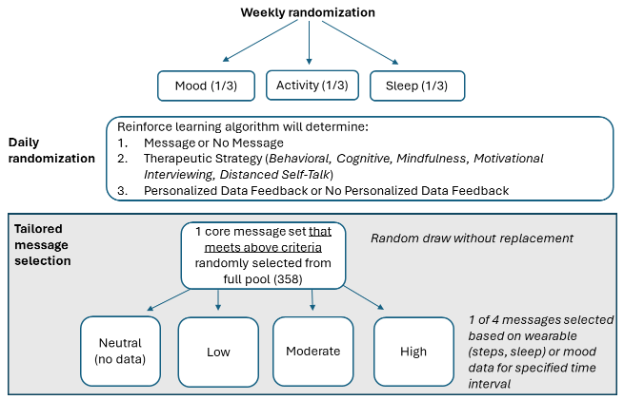
\includegraphics[width=\linewidth]{assets/study_design_2025.png}

  \item Figure 2 -- 2024 IHS Study Design
  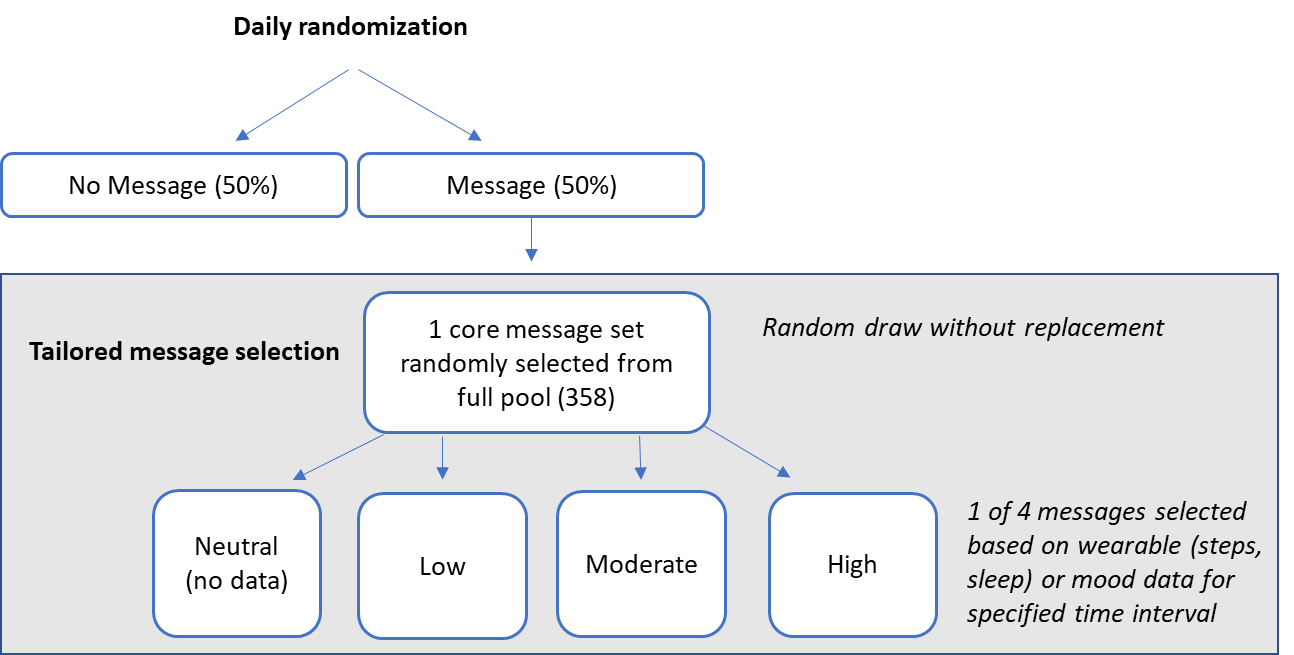
\includegraphics[width=\linewidth]{assets/study_design_2024.png}

  \item Table 2 -- Table of Cumulative Magnitude of Effects and P-Values
  \vspace{1.5em}
  
  \renewcommand{\arraystretch}{1.4}
  \begin{tabularx}{\textwidth}{|>{\raggedright\arraybackslash}X
                              |>{\centering\arraybackslash}X
                              |>{\centering\arraybackslash}X|}
  \hline
  \centering Intervention
    & Cumulative Magnitude of Effect
    & P-Value \\
  \hline
  Notification            &  &  \\
  \hline
  \quad Mindfulness       &  &  \\
  \hline
  \quad \ldots            & \ldots & \ldots \\
  \hline
  No Notification         &  &  \\
  \hline
  \end{tabularx}
  \renewcommand{\arraystretch}{1}
    

  \item Figure 3 -- Distribution of Effects
  
  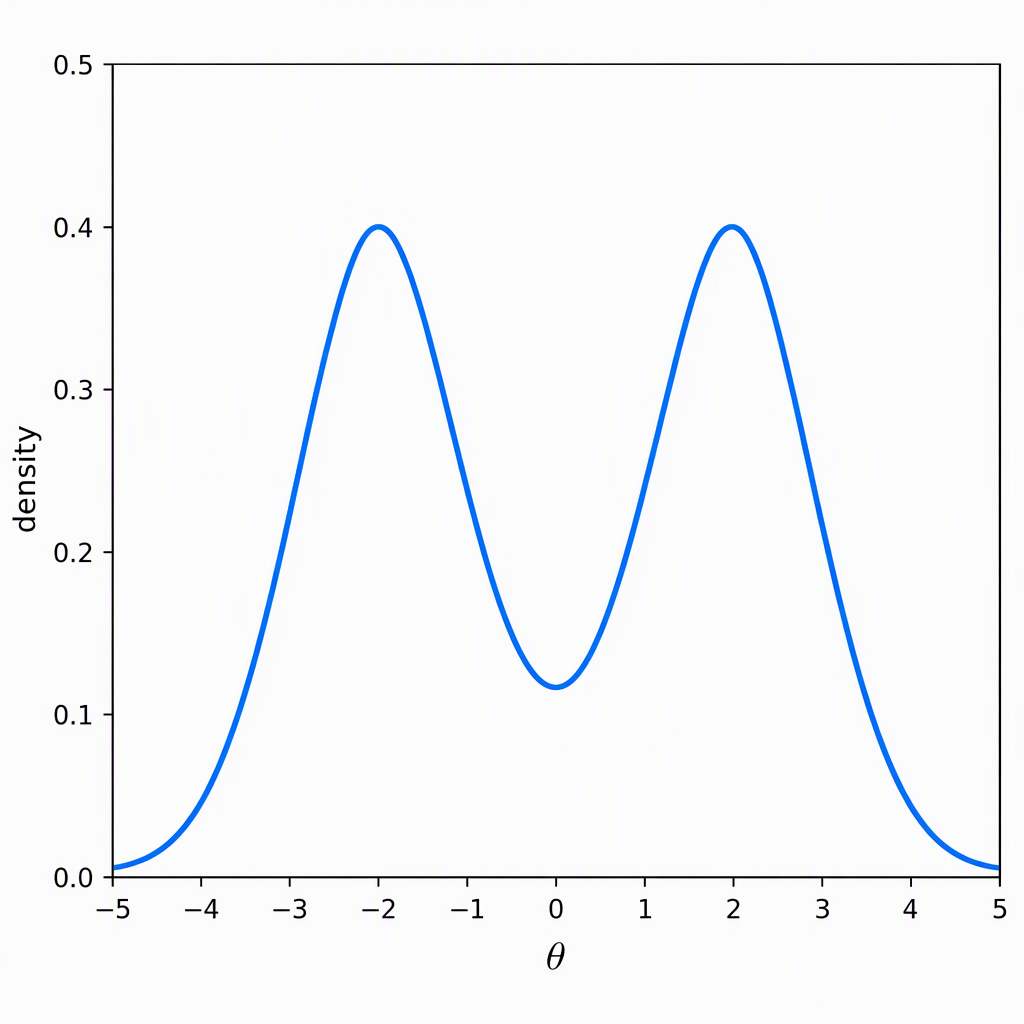
\includegraphics[width=0.4\linewidth]{assets/effect_distribution_example.png}

  \item Figure 4 -- Effect vs Baseline Characteristic
  
  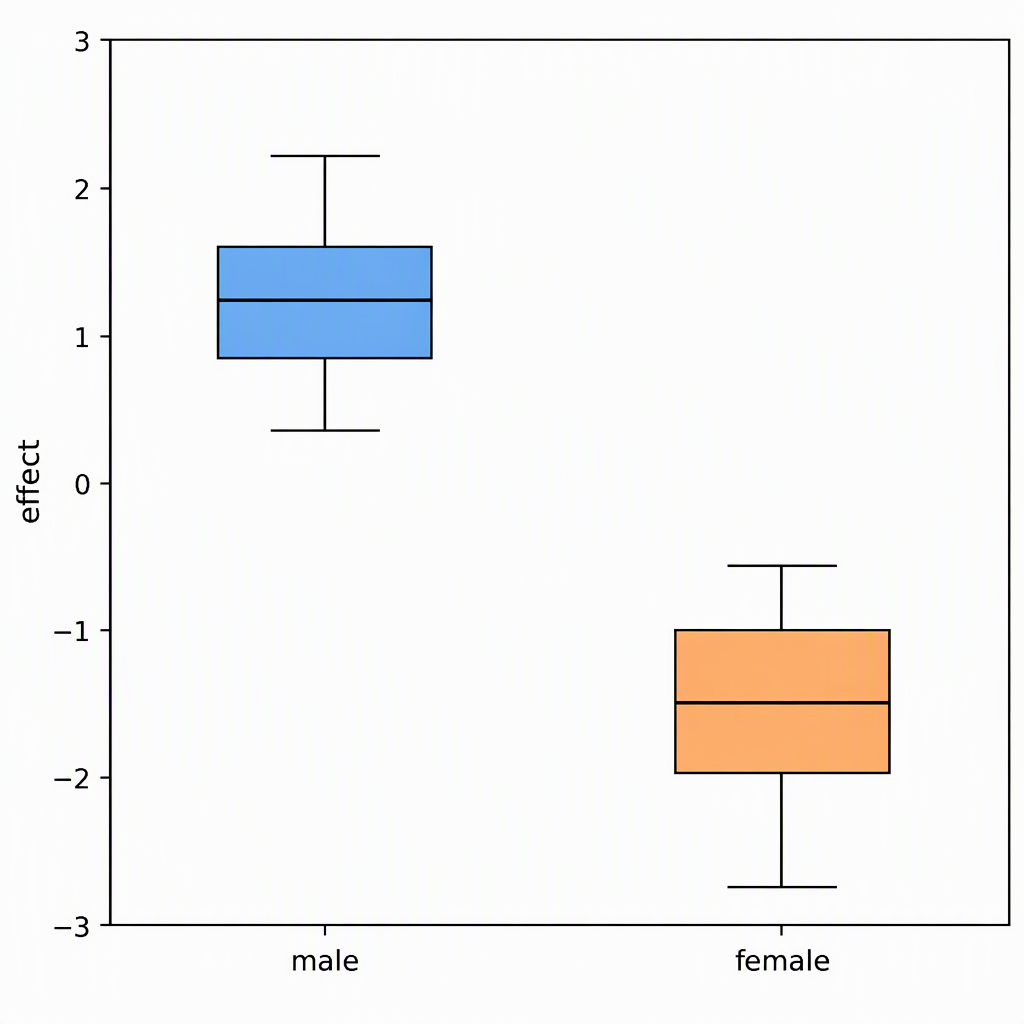
\includegraphics[width=0.4\linewidth]{assets/effect_vs_characteristic_example.png}
\end{enumerate}


% References
\bibliographystyle{plain}
\bibliography{proposal}

\end{document}
